% !Mode:: "TeX:UTF-8"

\chapter{张力分配算法设计与仿真比较}

\section{引言}

张力分配是绳驱并联机器人控制实现中的关键环节。对于本文研究的平面四绳三自由度系统而言，末端平台期望广义力一旦确定，系统需要进一步求解各绳的目标张力，并通过卷筒半径映射为各电机的目标力矩。由于绳索仅能承受拉力，且各绳张力还必须满足传动机构与传感器允许的上下界，因此张力分配问题本质上是一个带不等式约束的冗余力分配问题\cite{gouttefarde2007wrench,phan2021wrenchclosure,tao2021tensiondistribution}。

上一章已经建立了由末端位姿误差到广义力修正量、再到张力增量的控制链路，但该链路并未进一步讨论在冗余驱动条件下如何从无穷多组可行张力解中选取更适合样机实现的一组。不同的张力分配算法会直接影响各绳张力裕度、张力均匀性、实时性以及后续电机力矩控制难度。尤其对于本文高动态连续旋转场景而言，若张力分配结果过于接近上下边界，则会增加松绳风险或造成执行器饱和；若张力波动过大，则会放大电机内环负担并削弱末端加速度输出品质\cite{cao2023realtimetension,song2024realtimemethod,wang2024dynamictension}。

基于上述考虑，本章围绕张力分配问题展开专门分析。首先建立本文样机的张力分配数学模型，并推导单冗余系统的张力通解及其可行区间。随后，结合仿真程序中的实现方式，分别给出最小范数优化基线法、重心法和解析中心法的构造过程。最后，在工作空间采样和典型轨迹工况下对三类算法进行对比，综合可行性、张力裕度、均匀性和实时性等指标确定本文后续采用的张力分配方案。

\section{张力分配问题建模}

\subsection{目标广义力与张力平衡关系}

对于平面四绳三自由度绳驱系统，末端平台在任务空间中的目标广义力可写为
\begin{equation}
  \bm w_p^\ast=\begin{bmatrix} F_x^\ast & F_y^\ast & M_z^\ast \end{bmatrix}^{\mathrm T}.\label{eq:ch5-target-wrench}
\end{equation}
根据第3章建立的结构矩阵，四根绳张力与末端平台广义力之间满足
\begin{equation}
  \bm W\bm f=\bm w_p^\ast, \label{eq:ch5-wrench-balance}
\end{equation}
其中，$\bm f=\begin{bmatrix} f_1 & f_2 & f_3 & f_4 \end{bmatrix}^{\mathrm T}$ 为四根绳索张力向量，$\bm W\in\mathbb R^{3\times 4}$ 为由绳索方向和力矩臂共同构成的结构矩阵。由于本文系统具有4根绳索和3个独立广义力分量，因此张力分配问题属于单冗余约束系统，其张力解一般并不唯一\cite{gouttefarde2007wrench,tao2021tensiondistribution}。

进一步考虑绳索单向受力和执行器能力限制，各绳张力还应满足
\begin{equation}
  f_{i,\min}\le f_i\le f_{i,\max},\qquad i=1,2,3,4, \label{eq:ch5-force-bound}
\end{equation}
式中，$f_{i,\min}$ 为第$i$根绳索为避免松绳而设置的最小预紧张力，$f_{i,\max}$ 为由电机、卷筒、绳索和传感器共同决定的允许最大张力。依据本文仿真参数，四根绳的下界统一取 $1.5\ \mathrm N$，上界统一取 $12\ \mathrm N$。

因此，本文张力分配问题可以统一描述为：在满足式\eqref{eq:ch5-wrench-balance}和式\eqref{eq:ch5-force-bound}的前提下，求取一组既能实现目标广义力、又适合实时控制与样机执行的张力向量 $\bm f$。

\subsection{张力分配评价目标}

仅以“存在一组可行张力解”为目标通常是不够的。对于实际样机系统，更合理的张力分配算法还应同时满足以下要求。

首先，分配结果应具有较好的边界裕度，即各绳张力尽量远离上下界。这样既可以降低因扰动导致的松绳风险，也能减小执行器饱和的可能性。其次，分配结果应尽量平衡各绳负载，避免某一根绳长期承担过大的张力。再次，算法应具有较好的实时性和计算稳定性，以适应闭环控制中的在线调用需求。最后，在轨迹跟踪过程中，张力变化不宜出现不必要的剧烈跳变，否则会增加单电机力矩控制负担并恶化末端加速度连续性\cite{cao2023realtimetension,song2024realtimemethod,wang2024dynamictension}。

基于上述考虑，本文后续仿真比较将重点围绕以下指标展开：一是可行性，即给定工况下算法是否能够得到满足上下界约束的张力解；二是最小张力裕度，即各绳对边界的最小剩余距离；三是张力均匀性，即各绳张力相对均值的离散程度；四是在线求解复杂度，即算法在单次求解时的实现难度和计算量。通过这些指标的综合比较，可为后续控制实验选择更合适的张力分配方案。

\section{单冗余张力通解与可行区间推导}

\subsection{张力通解表达式}

对式\eqref{eq:ch5-wrench-balance}而言，结构矩阵 $\bm W$ 的列数大于行数，因此其解空间可分解为特解与零空间解之和。设 $\bm f_p$ 为满足
\begin{equation}
  \bm W\bm f_p=\bm w_p^\ast \label{eq:ch5-fp}
\end{equation}
的一组特解，则张力通解可写为
\begin{equation}
  \bm f=\bm f_p+\bm n_s\lambda, \label{eq:ch5-general-solution}
\end{equation}
其中，$\bm n_s\in\mathbb R^{4\times 1}$ 为结构矩阵零空间的一组单位基向量，满足
\begin{equation}
  \bm W\bm n_s=\bm 0, \label{eq:ch5-nullspace}
\end{equation}
$\lambda\in\mathbb R$ 为冗余自由度对应的标量参数。结合本文仿真程序的实现，特解采用广义逆形式求取，即
\begin{equation}
  \bm f_p=\bm W^\dagger \bm w_p^\ast, \label{eq:ch5-fp-pinv}
\end{equation}
其中，$\bm W^\dagger$ 为结构矩阵的 Moore--Penrose 广义逆。

式\eqref{eq:ch5-general-solution}表明，在给定目标广义力后，所有满足力平衡的张力向量均分布在一条一维仿射子空间上。此时张力分配问题可以转化为对标量参数 $\lambda$ 的求取问题，这也是本文后续重心法和解析中心法得以简化实现的基础。

进一步地，将式\eqref{eq:ch5-general-solution}写成分量形式可得
\begin{equation}
  f_i(\lambda)=f_{p,i}+\lambda n_{s,i},\qquad i=1,2,3,4. \label{eq:ch5-fi-lambda}
\end{equation}
这说明每根绳张力关于冗余参数 $\lambda$ 都呈线性变化，其斜率正是零空间向量 $\bm n_s$ 的对应分量 $n_{s,i}$。因此，当 $n_{s,i}>0$ 时，第 $i$ 根绳张力随 $\lambda$ 增大而增大；当 $n_{s,i}<0$ 时，第 $i$ 根绳张力随 $\lambda$ 增大而减小；若 $n_{s,i}=0$，则该绳张力与 $\lambda$ 无关。对于冗余驱动系统而言，这种“部分绳张力增大、部分绳张力减小”的现象并不矛盾，它恰好反映了在不改变目标广义力的前提下，张力沿零空间方向在各绳之间重新分配的过程。需要进一步说明的是，后文示意图中采用了“两条上升、两条下降”的典型画法，以便更直观地表现平面四绳系统中张力在不同绳之间的再分配关系；严格而言，各绳张力对 $\lambda$ 的升降趋势由零空间向量 $\bm n_s$ 各分量的符号决定，并不必然固定为两升两降。后文可行区间示意图中不同直线斜率的正负差异，正来源于这一点。

\subsection{上下界约束诱导的可行区间}

将式\eqref{eq:ch5-general-solution}代入张力上下界约束式\eqref{eq:ch5-force-bound}，对第$i$根绳有
\begin{equation}
  f_{i,\min}\le f_{p,i}+n_{s,i}\lambda\le f_{i,\max}, \label{eq:ch5-lambda-ineq}
\end{equation}
其中，$f_{p,i}$ 和 $n_{s,i}$ 分别为向量 $\bm f_p$ 和 $\bm n_s$ 的第$i$个分量。若 $n_{s,i}>0$，则可得
\begin{equation}
  \frac{f_{i,\min}-f_{p,i}}{n_{s,i}}\le \lambda\le \frac{f_{i,\max}-f_{p,i}}{n_{s,i}}. \label{eq:ch5-lambda-positive}
\end{equation}
若 $n_{s,i}<0$，则不等号方向翻转，可写为
\begin{equation}
  \frac{f_{i,\max}-f_{p,i}}{n_{s,i}}\le \lambda\le \frac{f_{i,\min}-f_{p,i}}{n_{s,i}}. \label{eq:ch5-lambda-negative}
\end{equation}
若 $n_{s,i}=0$，则第$i$根绳的张力与 $\lambda$ 无关，此时仅需判断 $f_{p,i}$ 是否已经满足上下界约束。

综合四根绳的约束后，标量 $\lambda$ 的全局可行区间可表示为
\begin{equation}
  \lambda_{\min}=\max_i\{\lambda_{i,\mathrm l}\},\qquad \lambda_{\max}=\min_i\{\lambda_{i,\mathrm u}\}, \label{eq:ch5-lambda-bounds}
\end{equation}
其中，$\lambda_{i,\mathrm l}$ 和 $\lambda_{i,\mathrm u}$ 分别表示由第$i$根绳张力上下界诱导出的局部下界和局部上界。当满足
\begin{equation}
  \lambda_{\min}\le \lambda_{\max} \label{eq:ch5-feasible-interval}
\end{equation}
时，说明当前目标广义力存在满足全部张力约束的可行分配解；否则说明该工况下无可行张力分配，需要通过重新规划目标广义力或修改工作点来处理\cite{gouttefarde2007wrench,phan2021wrenchclosure}。

\begin{figure}[htbp]
  \centering
  \begin{tikzpicture}[
    >=Stealth,
    line width=0.9pt,
    font=\small
  ]
    % 坐标轴
    \draw[->] (-1,0) -- (10.2,0) node[below] {$\lambda$};
    \draw[->] (-1,0) -- (-1,6.1) node[left] {$f_i(\lambda)$};

    % 可行区间阴影
    \fill[gray!15] (2,0) rectangle (8,5.8);
    \draw[dashed] (2,0) -- (2,5.8);
    \draw[dashed] (8,0) -- (8,5.8);
    \node[below] at (2,0) {$\lambda_{\min}$};
    \node[below] at (8,0) {$\lambda_{\max}$};

    % 上下界
    \draw[dashed] (-0.8,1.0) -- (9.6,1.0);
    \draw[dashed] (-0.8,5.0) -- (9.6,5.0);
    \node[left] at (-1,1.0) {$f_{\min}$};
    \node[left] at (-1,5.0) {$f_{\max}$};

    % 四根绳张力直线
    \draw[blue]   (0.7,1.6) -- (9.2,3.9);
    \draw[red]    (0.7,4.2) -- (9.2,1.8);
    \draw[teal!70!black] (0.7,2.2) -- (9.2,4.3);
    \draw[orange!90!black] (0.7,4.95) -- (9.2,2.4);

    % 线标注放左侧和右侧分开
    \node[blue, anchor=east] at (0.65,1.6) {$f_1(\lambda)$};
    \node[red, anchor=east] at (0.65,4.2) {$f_2(\lambda)$};
    \node[teal!70!black, anchor=west] at (9.25,4.3) {$f_3(\lambda)$};
    \node[orange!90!black, anchor=west] at (9.25,2.4) {$f_4(\lambda)$};

    % 重心解与解析中心解
    \draw[dashdotted] (5.0,0) -- (5.0,5.8);
    \draw[dashdotted] (5.8,0) -- (5.8,5.8);
    \fill (5.0,0) circle (1.2pt);
    \fill (5.8,0) circle (1.2pt);
    \node[below] at (5.0,0) {$\lambda_{\mathrm{bary}}$};
    \node[below] at (5.8,0) {$\lambda_{\mathrm{ac}}$};

    % 最小张力裕度示意：黑色箭头表示最小裕度，灰色箭头表示另一侧边界距离
    \draw[<->] (5.0,3.66) -- (5.0,5.0);
    \draw[<->, gray!70] (5.0,1.0) -- (5.0,2.78);
    \node[left] at (4.92,4.33) {$\eta_{\mathrm{bary}}$};

    \draw[<->] (5.8,3.44) -- (5.8,5.0);
    \draw[<->, gray!70] (5.8,1.0) -- (5.8,2.8);
    \node[right] at (5.88,4.21) {$\eta_{\mathrm{ac}}$};

    % 可行区间标题
    \node at (5,5.45) {可行区间};

  \end{tikzpicture}
  \caption{单冗余张力通解与冗余参数可行区间示意图}
  \label{fig:ch5-lambda-feasible-interval}
\end{figure}



如\cref{fig:ch5-lambda-feasible-interval}所示，由式 $\bm f(\lambda)=\bm f_p+\lambda\bm n_s$ 可知，各绳张力关于冗余参数 $\lambda$ 呈线性变化。张力上下界进一步将 $\lambda$ 限制在区间 $[\lambda_{\min},\lambda_{\max}]$ 内，不同张力分配算法的差异本质上体现为在该可行区间内选取不同的 $\lambda$。对于本文4绳3自由度系统，张力分配问题最终可简化为在一维可行区间内选取最合适的 $\lambda$。

需要特别说明的是，图中的“张力裕度”不是指 $\lambda$ 到区间端点 $\lambda_{\min}$、$\lambda_{\max}$ 的横向距离，而是指在某个给定 $\lambda$ 处，各绳张力值到上下边界 $f_{\min}$、$f_{\max}$ 的最小纵向距离。换言之，当在图中固定某一个 $\lambda$ 并作竖线时，该竖线与四条 $f_i(\lambda)$ 直线的交点分别给出四根绳的张力值；这些交点中距离 $f_{\min}$ 或 $f_{\max}$ 最近的那个距离，就是该解对应的最小张力裕度。图中的黑色箭头对应最小张力裕度，灰色箭头表示同一 $\lambda$ 处到另一侧边界的剩余距离。若某一解点附近的交点更靠近上下边界，则说明该解更容易贴近约束；若交点整体远离上下边界，则说明该解保留了更大的安全余量。

图中的下标“bary”表示重心法（barycenter）对应的取点位置，因此 $\lambda_{\mathrm{bary}}=(\lambda_{\min}+\lambda_{\max})/2$，即严格取可行区间中点作为分配参数时得到的冗余参数取值；下标“ac”表示解析中心法（analytic center）对应的取点位置，因此 $\lambda_{\mathrm{ac}}$ 表示通过对数势函数或等价的一维搜索得到的解析中心解。之所以图中分别选取这两个 $\lambda$，是因为它们正对应本文后续重点比较的两类解析分配策略：前者直接取区间中点，后者主动远离约束边界。通过在这两个代表点上比较最小张力裕度，便可以直观说明为什么解析中心法通常能比重心法保留更大的安全余量。因此，后续不同算法之间的差异，不仅体现为它们在可行区间中的取点位置不同，更体现为这些取点所对应的最小张力裕度和边界敏感性不同。

\section{张力分配算法构造}

\subsection{最小范数优化基线法}

为便于与后续快速解析方法进行比较，本文首先保留一种基于数值优化的最小范数法作为基线方案。其基本思想是在满足力平衡和张力上下界约束的前提下，求取欧氏范数最小的张力向量，即
\begin{equation}
  \min_{\bm f}\ J_1(\bm f)=\|\bm f\|_2, \label{eq:ch5-minnorm-obj}
\end{equation}
约束条件为
\begin{equation}
  \bm W\bm f=\bm w_p^\ast, \qquad\bm f_{\min}\le \bm f\le \bm f_{\max}.\label{eq:ch5-minnorm-eq}
\end{equation}
该方法与本文仿真代码中 `fmincon` 基线实现一致，其优点是建模直接、易于扩展到更一般的目标函数；缺点是每次求解均需进行约束优化，实时性受优化器初始化和迭代过程影响较大。对于本文这种仅有一维冗余的系统而言，若继续采用通用优化器，会在一定程度上浪费结构信息。

\subsection{重心法}

重心法利用了单冗余系统可行解集在 $\lambda$ 轴上退化为闭区间这一特点。设可行区间为 $[\lambda_{\min},\lambda_{\max}]$，则取其中点
\begin{equation}
  \lambda_c=\frac{\lambda_{\min}+\lambda_{\max}}{2}. \label{eq:ch5-barycenter-lambda}
\end{equation}
再代入式\eqref{eq:ch5-general-solution}即可得到重心法张力解
\begin{equation}
  \bm f_{\mathrm{bar}}=\bm f_p+\bm n_s\lambda_c. \label{eq:ch5-barycenter-force}
\end{equation}
对于一维区间而言，中点就是几何意义下的重心，因此该方法实现简单、计算量极小，并且能够在一定程度上使解远离边界。本文仿真程序中的 `bary\_center\_planar` 即采用这一思想\cite{tao2021tensiondistribution}。不过，重心法只利用了区间端点信息，并未显式考虑各绳张力对上下界的实际距离，因此当不同绳对约束的敏感程度差异较大时，所得结果未必具有最优边界裕度。

\subsection{解析中心法}

为进一步提高张力分配的边界鲁棒性，本文采用解析中心法作为主要候选方案。其思想是在可行域内部构造对数势函数，使求得的解尽量远离各约束边界。对本文问题，可定义目标函数为
\begin{equation}
  J_2(\bm f)=-\sum_{i=1}^{4}\ln\left(f_i-f_{i,\min}\right)-\sum_{i=1}^{4}\ln\left(f_{i,\max}-f_i\right). \label{eq:ch5-barrier}
\end{equation}
将式\eqref{eq:ch5-general-solution}代入后，上式可进一步化为仅关于 $\lambda$ 的一维优化问题
\begin{equation}
  \min_{\lambda\in(\lambda_{\min},\lambda_{\max})} J_2\bigl(\bm f_p+\bm n_s\lambda\bigr). \label{eq:ch5-barrier-lambda}
\end{equation}
由于对数势函数在边界附近趋于无穷大，因此其极小值对应的解会自然趋向可行域内部，从而获得更好的上下界裕度。本文程序中先根据式\eqref{eq:ch5-lambda-bounds}得到 $\lambda$ 的可行区间，再在略微收缩后的开区间内采用一维搜索求解最优 $\lambda^\ast$，最终张力解写为
\begin{equation}
  \bm f_{\mathrm{ac}}=\bm f_p+\bm n_s\lambda^\ast. \label{eq:ch5-ac-force}
\end{equation}
与重心法相比，解析中心法仍保持了一维求解的低复杂度，但能够更充分地利用所有约束边界信息，因此更有利于提高张力分配的稳定性与鲁棒性\cite{cao2023realtimetension,song2024realtimemethod,wang2024dynamictension}。

\section{仿真比较与算法选择}

\subsection{比较工况与评价指标}

为比较不同张力分配算法在本文样机上的适用性，仿真从两类工况展开。第一类为工作空间离散采样工况，即在典型平面工作区域内对末端位置进行网格化采样，并在零加速度条件下求解静态张力分布，用于观察不同算法的可行区域和张力边界裕度。第二类为典型轨迹工况，即将算法嵌入给定末端轨迹的连续求解过程中，对比各算法在实际运动过程中的张力变化规律和实时计算特性。本文所采用的典型轨迹为平动圆轨迹与姿态转动相结合的复合轨迹：末端平动部分沿半径为 $0.1\,\mathrm{m}$ 的圆轨迹运动，姿态角则按预设光滑轨迹连续变化，从而在保持几何特征清晰的同时兼顾位置与姿态耦合变化。

针对上述工况，本文采用以下指标进行比较：一是可行性指标，即采样点或轨迹点是否能得到满足约束的张力解；二是最小边界裕度指标
\begin{equation}
  \eta_{\min}=\min_i\left\{\min\left(f_i-f_{i,\min},\ f_{i,\max}-f_i\right)\right\}, \label{eq:ch5-margin}
\end{equation}
其值越大，说明当前张力解离边界越远；三是张力均匀性指标
\begin{equation}
  \sigma_f=\sqrt{\frac{1}{4}\sum_{i=1}^{4}\left(f_i-\bar f\right)^2},\qquad \bar f=\frac{1}{4}\sum_{i=1}^{4}f_i, \label{eq:ch5-sigmaf}
\end{equation}
其值越小，说明各绳张力分布越均衡；四是张力变化率连续性，即考察张力曲线的一阶导数或离散差分在时间上的平滑程度。若目标张力本身虽保持连续，但其一阶导数在局部时刻发生突变，则会导致目标力矩变化率骤增，不利于后续单电机内环的平滑执行；五是在线实现难度，即单次求解所需的计算步骤和对初值的敏感程度。

\subsection{工作空间采样下的张力分布比较}

在工作空间离散采样工况下，三类算法都可用于求解静态张力分配，但它们在可行区边界附近的表现存在明显差异。最小范数基线法能够得到满足约束的解，但由于其目标函数主要追求整体张力范数较小，求解结果在某些采样点上会更接近张力下界。重心法的求解结果具有较好的计算稳定性，但其边界裕度主要由区间中点决定，在局部几何条件变化较快时不一定始终保持最优。相比之下，解析中心法通过对数势函数主动远离上下边界，通常能够在相同目标广义力下保留更大的最小张力裕度。

\begin{figure}[htbp]
  \centering
  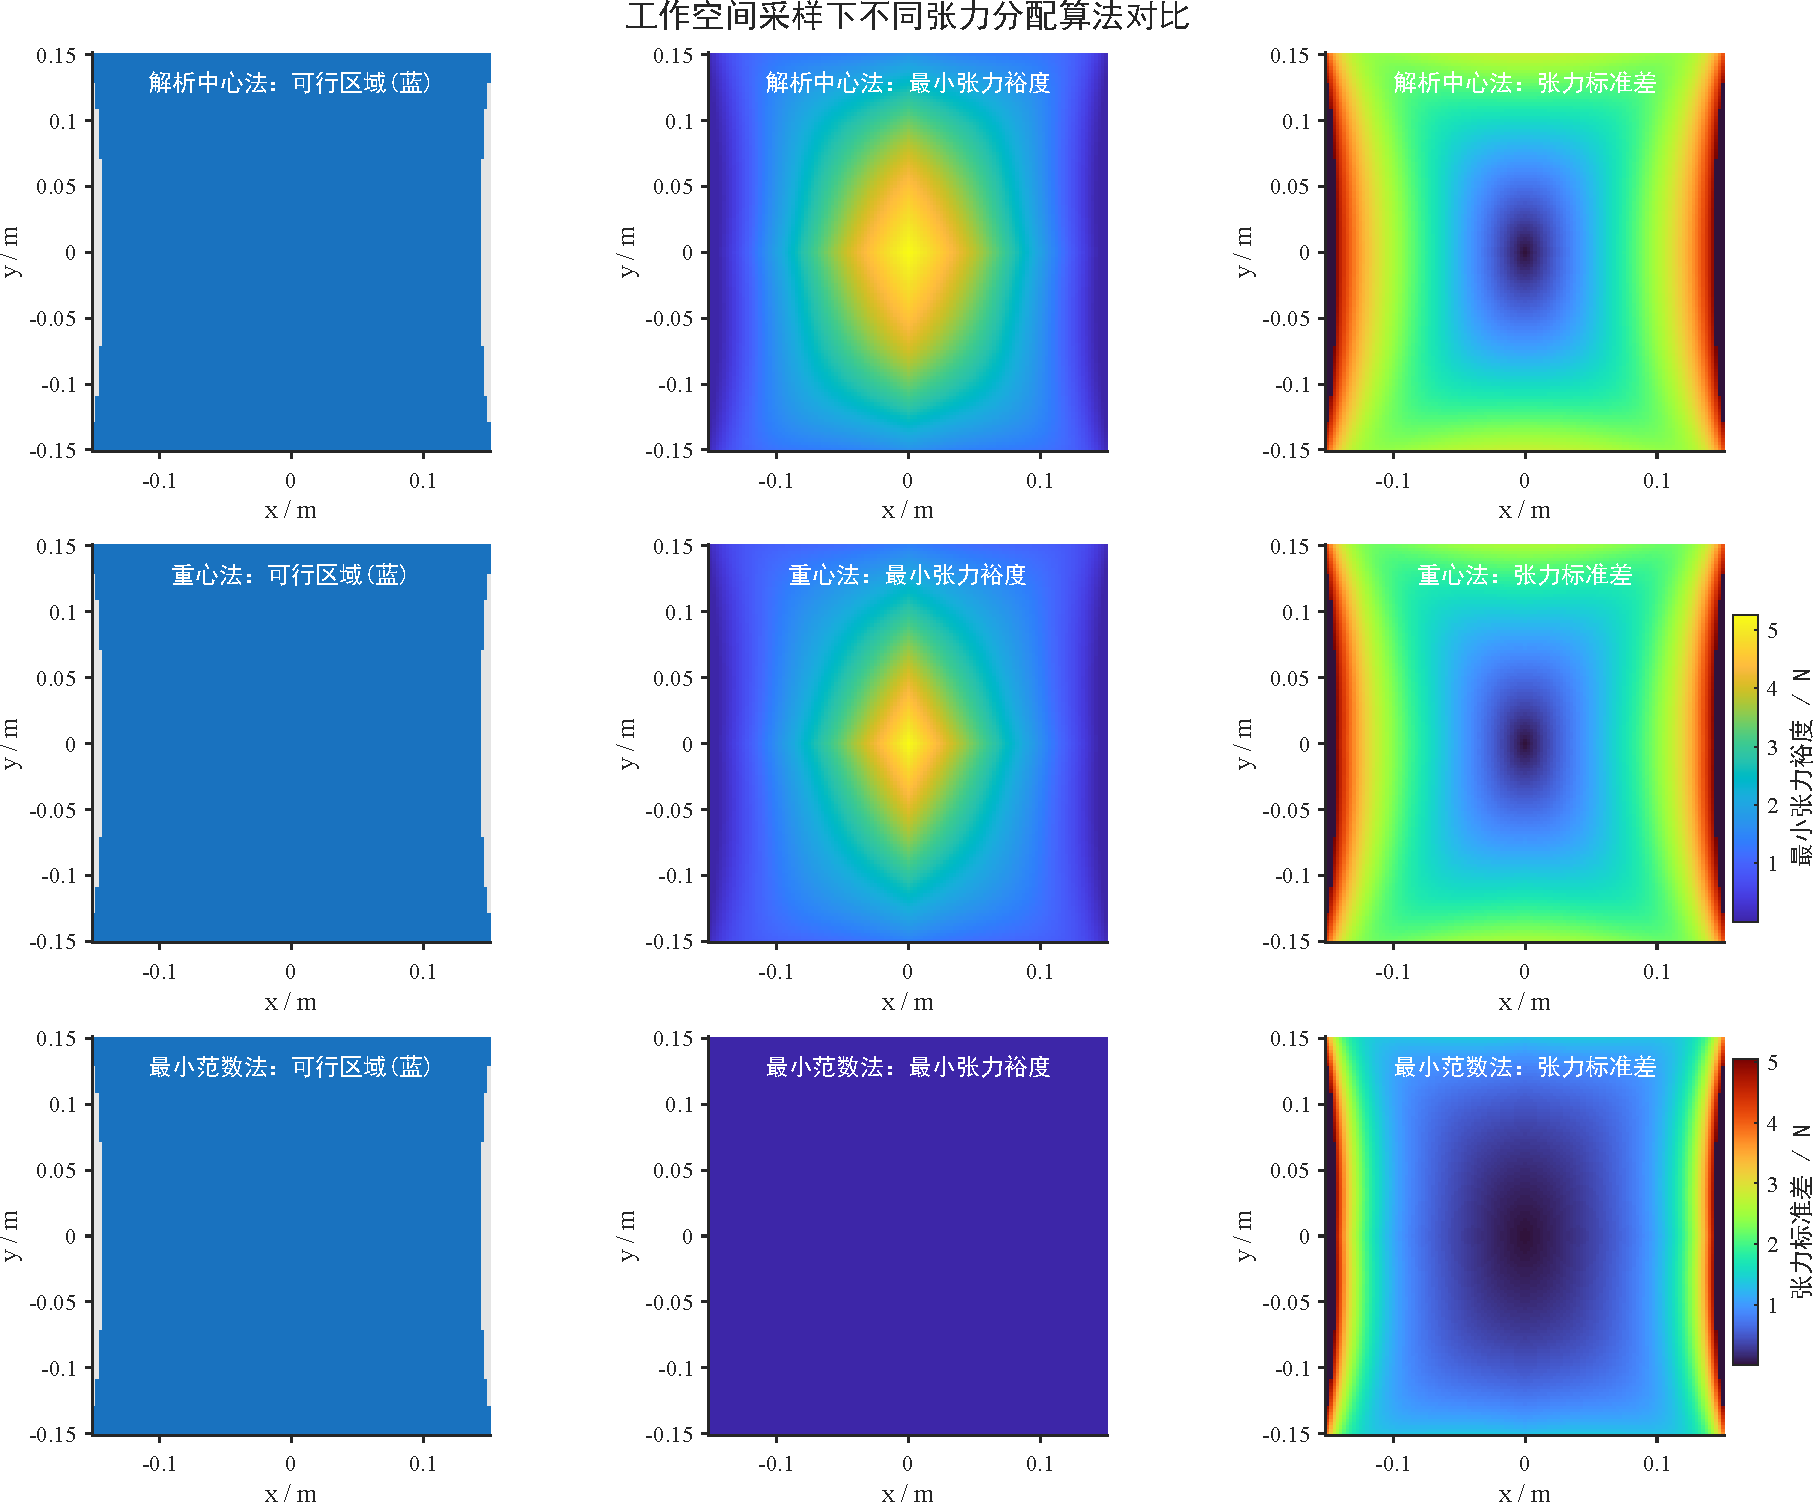
\includegraphics[width=0.95\textwidth]{figures/工作空间张力分配算法对比图.pdf}
  \caption{工作空间采样下不同张力分配算法的对比}
  \label{fig:ch5-workspace-compare}
\end{figure}

如\cref{fig:ch5-workspace-compare}所示，在平面内保持末端平台静止情况下进行求解，该图按列分别给出了三类指标：左列为可行区域分布，中列为最小张力裕度分布，右列为张力标准差分布。从左列可以看出,三种算法在本文工作空间范围内的可行区域总体接近，说明可行性首先主要受机构几何构型和张力上下界约束决定，而不是由区间内具体取点准则决定。中列结果表明，解析中心法在大部分采样区域内均获得了最大的最小张力裕度，重心法次之，而最小范数法几乎在整个工作空间内都接近张力下界，其最小张力裕度接近于零。这说明最小范数法虽然能够给出数值可行解，但其解通常贴近边界，不利于样机系统保留足够的抗扰余量。

右列结果进一步给出了三种算法的张力均匀性差异。三类算法均表现出“工作空间中心区域张力标准差较小、靠近边界时张力标准差增大”的共同规律，这是由于末端平台靠近边界时部分绳索需要承担更高载荷所致。与解析中心法和重心法相比，最小范数法的张力标准差整体更小，说明其更倾向于压低整体张力水平；但结合中列可知，这种“更均匀”是以明显压缩张力边界裕度为代价实现的。此外，最小范数法在每个采样点都需要调用数值优化器，计算耗时显著高于重心法和解析中心法，不利于后续控制中的在线实现。综合边界裕度、张力均匀性与计算速度三方面指标，解析中心法在保持工作空间可行性的同时，为后续控制和实验留出了更充足的安全张力余量，因此更适合作为本文后续张力分配的默认方案。

\subsection{典型轨迹工况下的张力变化比较}
\begin{figure}[htbp]
  \centering
  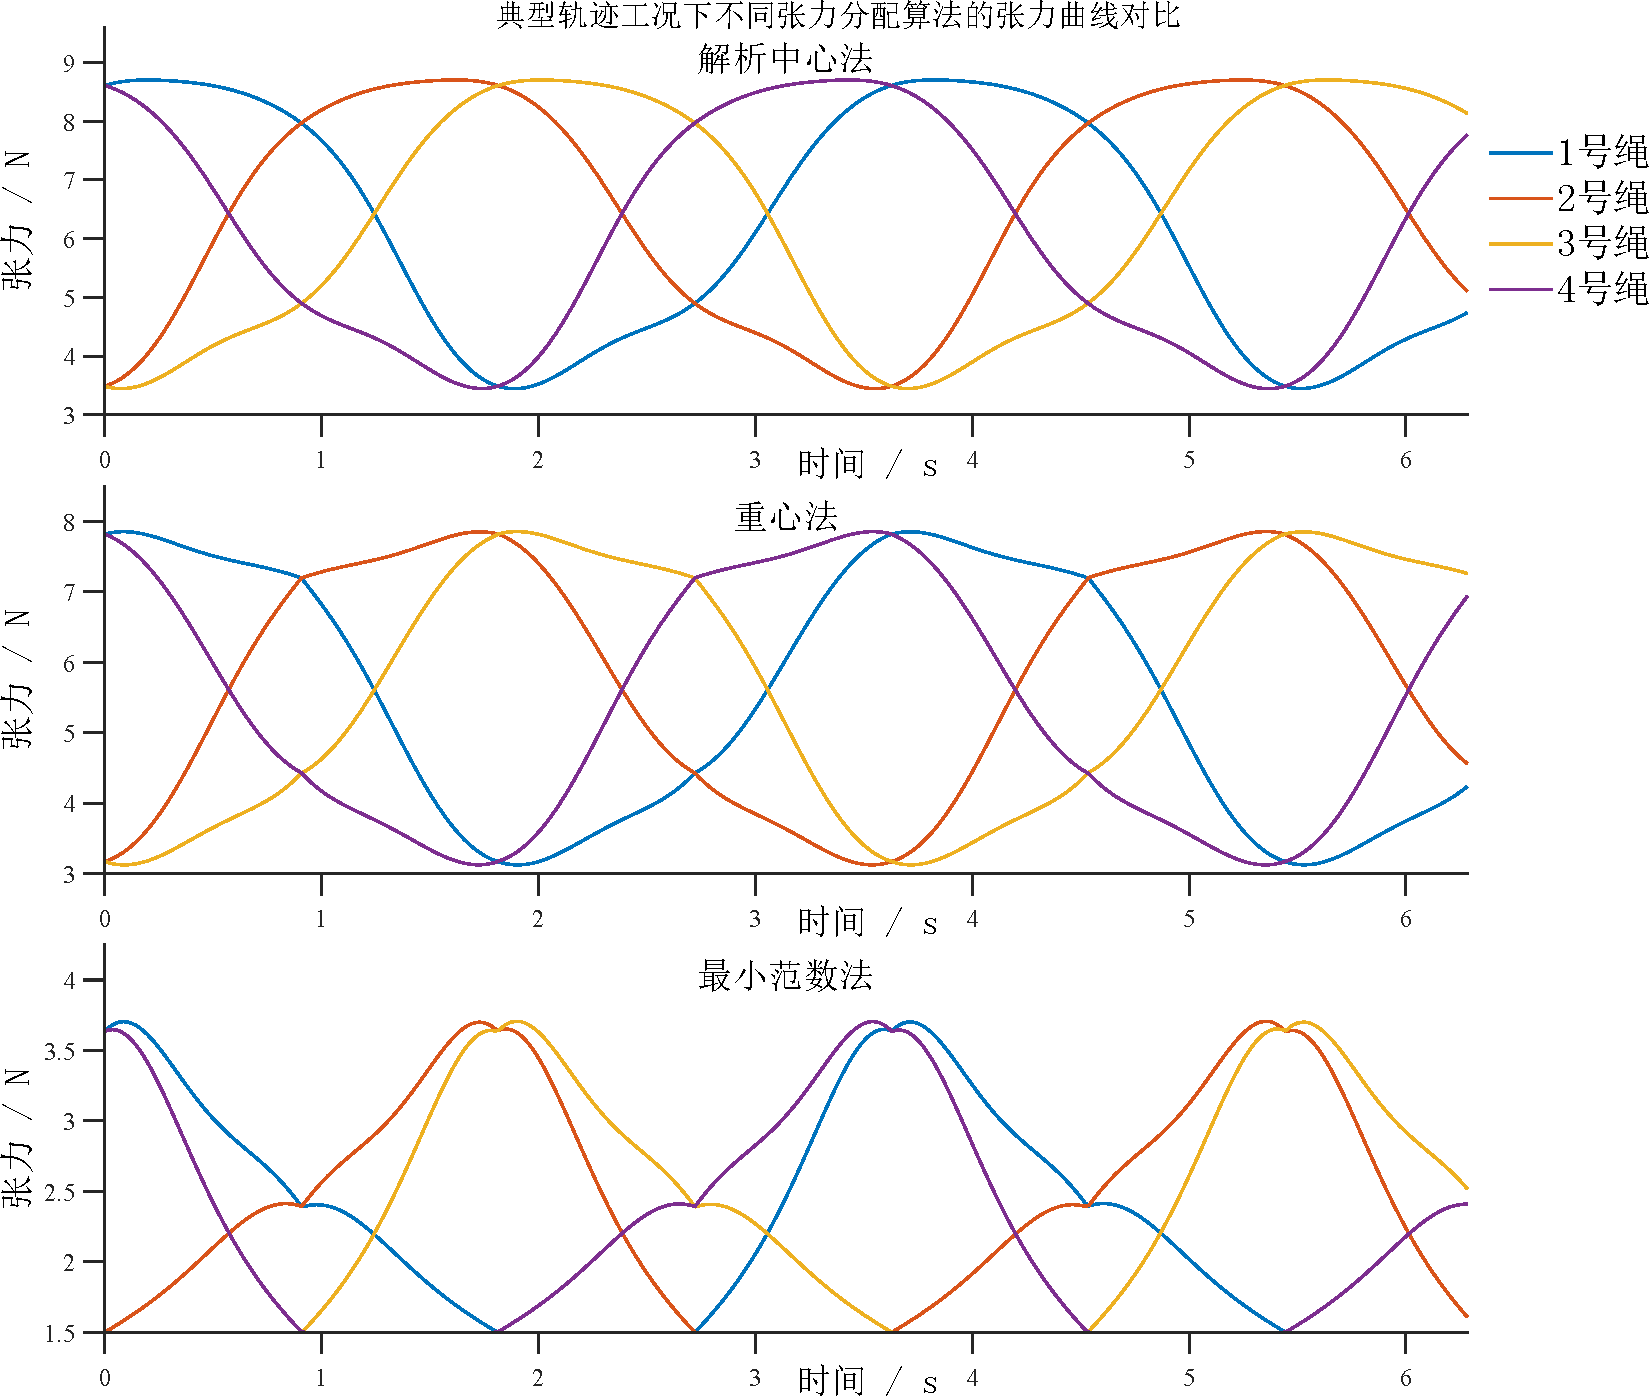
\includegraphics[width=0.92\textwidth]{figures/典型轨迹工况下不同张力分配算法张力曲线对比图.pdf}
  \caption{典型轨迹工况下不同张力分配算法的张力曲线对比}
  \label{fig:ch5-trajectory-compare}
\end{figure}
在典型轨迹工况下，算法优劣不仅体现在单个时刻的边界裕度上，还体现在整段运动中的张力平滑性、张力变化率连续性与可实现性上。对于本文样机而言，若张力分配结果在相邻时刻之间跳变较大，或虽然张力曲线本身连续但一阶导数存在明显突变，则都会直接增加单电机力矩内环的调节负担，并可能引起末端加速度输出的附加波动。最小范数法由于每一时刻均独立调用优化器求解，不仅在边界切换附近可能出现较明显的数值波动，而且在活动约束集合发生变化时更容易表现出张力一阶导数的不连续，同时整体计算耗时也更长；重心法由于取区间中点，整体较为平稳，且计算量极小，但在某些时刻可能牺牲部分边界裕度；解析中心法则在保持平滑性的同时兼顾了对边界的排斥作用，并保持了较好的实时性，更适合用于在线控制中的张力前馈与闭环修正。

如\cref{fig:ch5-trajectory-compare}所示，三种算法得到的张力曲线整体上都能保持连续，但细节差异依然明显。解析中心法在整段轨迹内保持了较好的张力裕度，其四根绳张力变化较为平滑；重心法虽然总体趋势与解析中心法接近，但在部分区段仍出现了较明显的折点，表明其张力一阶导数存在局部突变；最小范数法则由于求解结果长期贴近张力下界，且在活动约束切换处对优化结果更为敏感，因此不仅边界裕度较小，而且张力变化率的突变现象更为明显。

\begin{figure}[htbp]
  \centering
  \subfigure[最小范数法\label{fig:ch5-df-minnorm}]{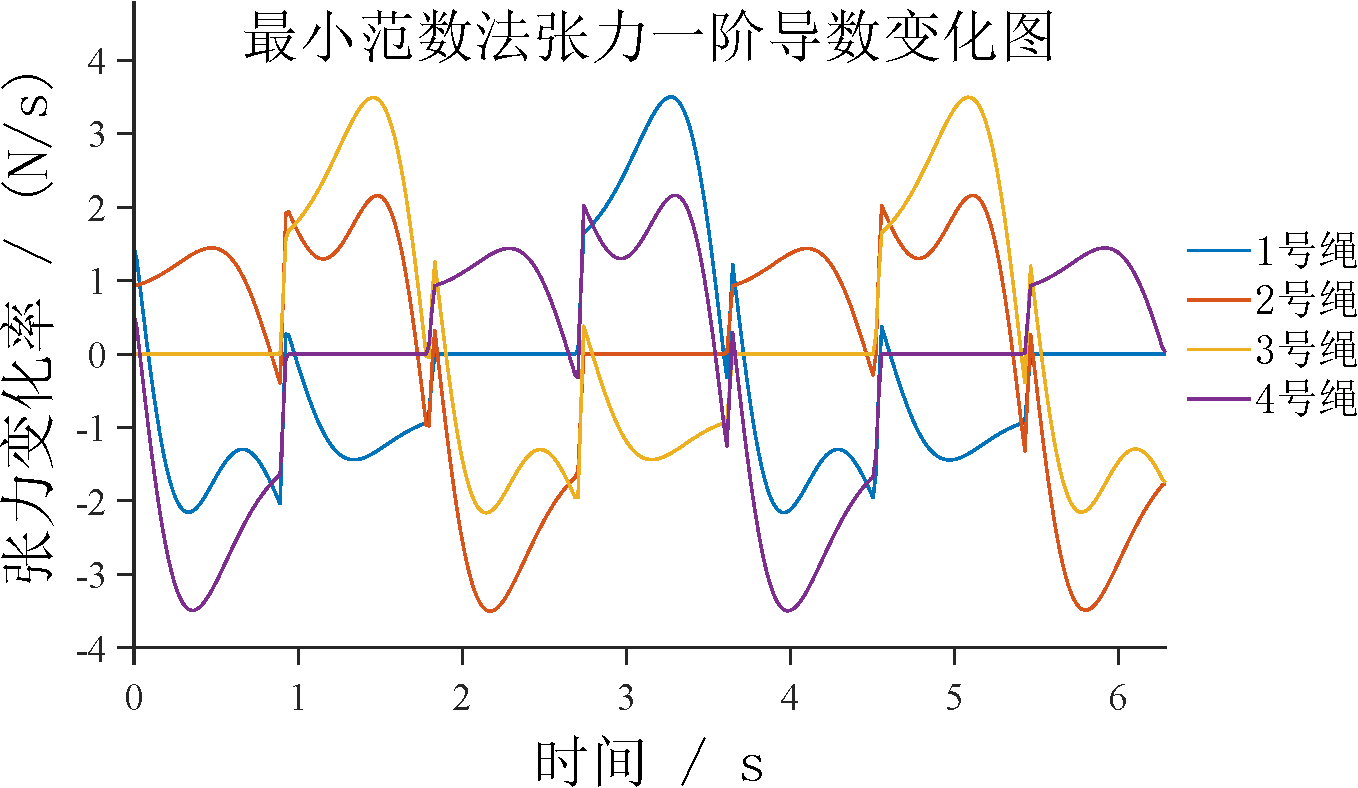
\includegraphics[width=0.48\textwidth]{figures/最小范数法张力一阶导数变化图.pdf}}
  \hfill
  \subfigure[重心法\label{fig:ch5-df-bary}]{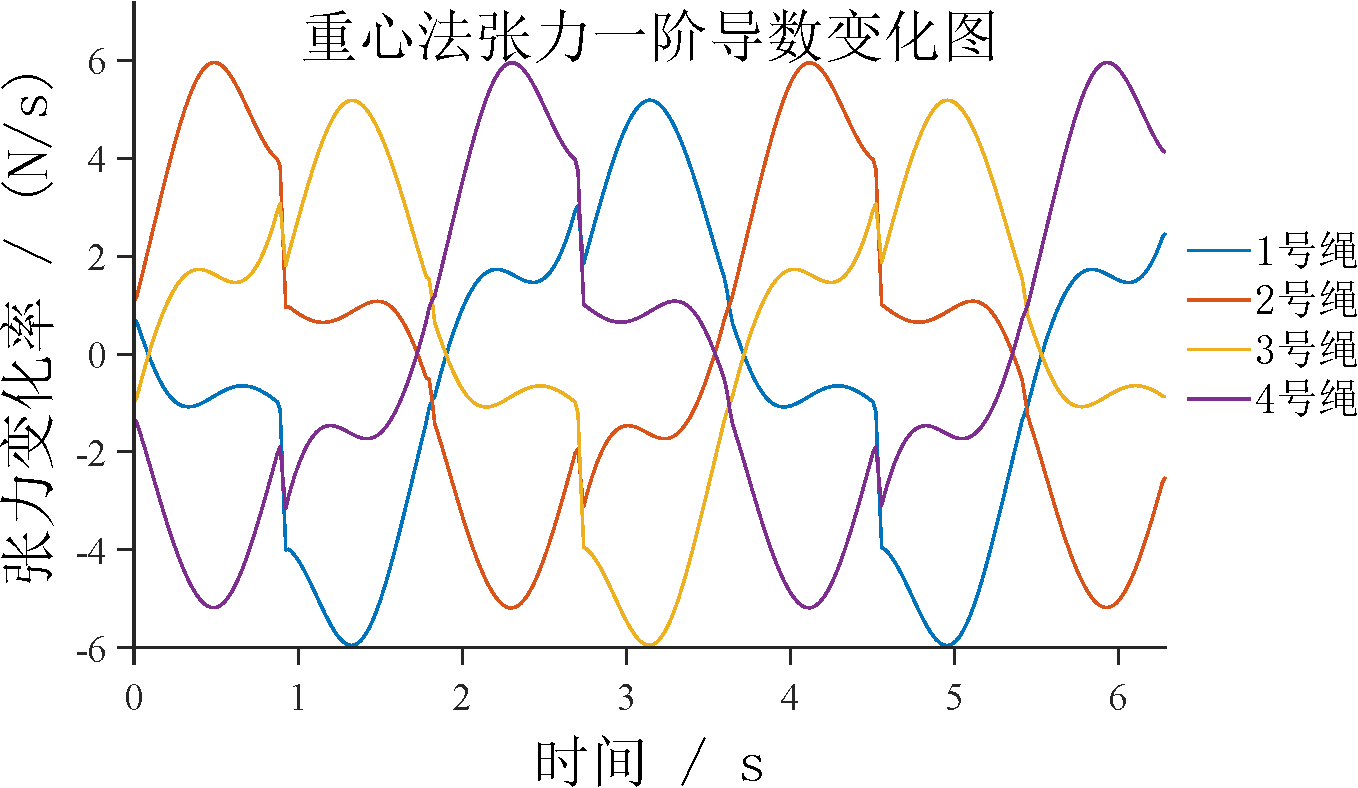
\includegraphics[width=0.48\textwidth]{figures/重心法张力一阶导数变化图.pdf}}

  \vspace{0.6em}

  \subfigure[解析中心法\label{fig:ch5-df-analytic}]{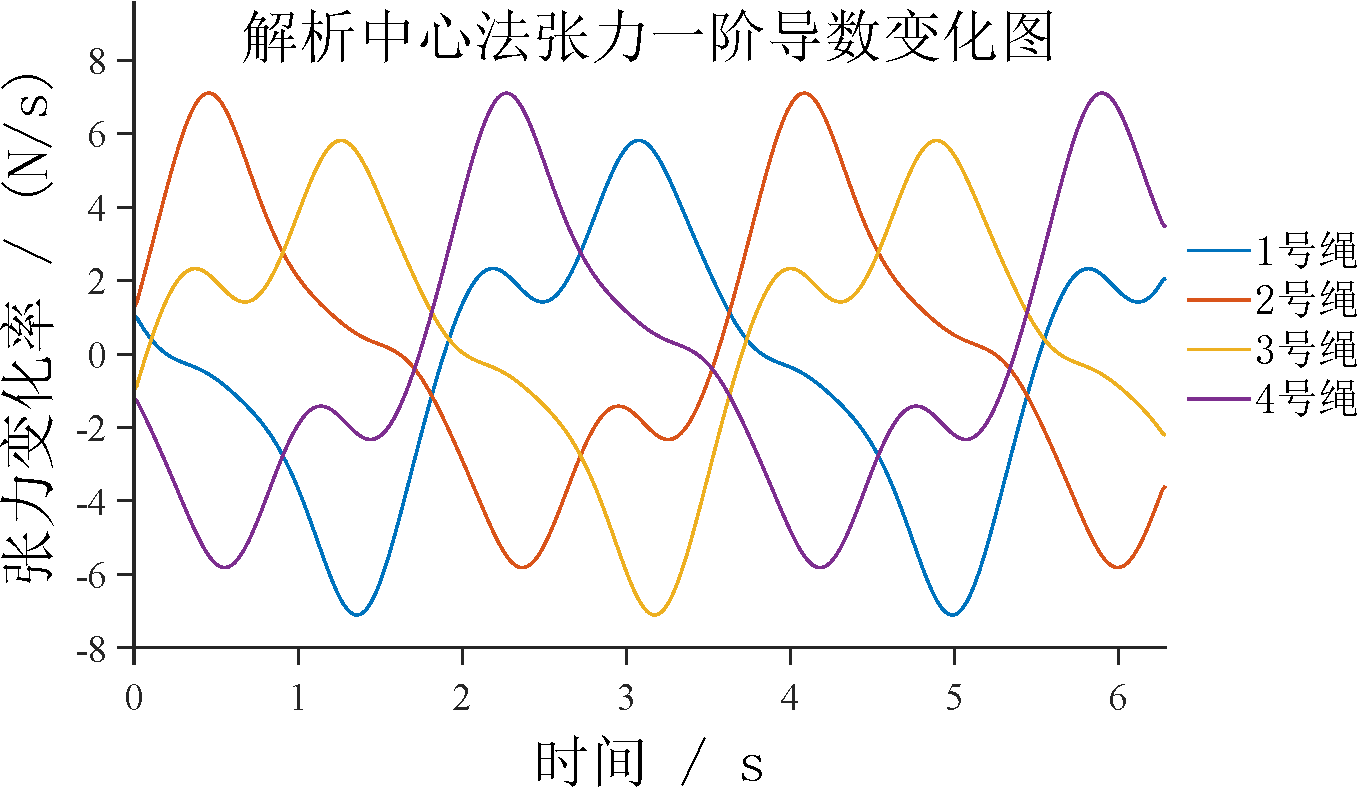
\includegraphics[width=0.48\textwidth]{figures/解析中心法张力一阶导数变化图.pdf}}
  \caption{典型轨迹工况下不同张力分配算法的一阶导数对比}
  \label{fig:ch5-trajectory-derivative}
\end{figure}

如\cref{fig:ch5-trajectory-derivative}所示，解析中心法对应的张力一阶导数整体较为平滑，仅在局部时刻出现较小波动；重心法的一阶导数已经表现出一定程度的局部突变；最小范数法的一阶导数突变最为明显，说明虽然其张力曲线本身连续，但对时间的一阶连续性很差。对于本文后续单电机力矩内环和末端加速度输出而言，这类导数突变会直接转化为更剧烈的目标力矩变化率，从而增加执行器调节负担，并可能引入附加抖振。

从轨迹工况的综合表现看，解析中心法在保证所有绳索维持正张力的同时，能够更有效地提升整体张力裕度，并减少边界附近的敏感性，其张力变化率也更有利于保持连续和平滑，因此其结果更适合作为后续控制章节中的目标张力生成方法。重心法可作为实现简单、实时性较好的近似方案，用于与解析中心法形成对照，但其导数层面仍存在局部突变；最小范数法则更适合作为数值优化基线，用于验证解析方法的合理性，而不宜作为本文完整样机的首选在线分配方法。

\subsection{算法选择与后续应用}

综合理论推导与仿真比较结果，本文后续张力分配算法选择解析中心法作为默认方案，理由主要包括以下三个方面。第一，解析中心法充分利用了单冗余系统可行区间的一维结构，计算复杂度低于逐点调用通用优化器的最小范数法，同时又比简单取中点的重心法具有更好的边界利用能力，因此更适合在线实现。第二，该方法能够显式增大解到张力上下界的距离，从而为扰动、模型误差和动态波动留出更大的安全余量。第三，与仅取几何中点的重心法相比，解析中心法对不同绳约束的综合考虑更充分，在工作空间边缘和高动态轨迹下通常能表现出更稳定的张力分布\cite{cao2023realtimetension,song2024realtimemethod,wang2024dynamictension}。

需要指出的是，本文所采用的解析中心法建立在“4绳3自由度、冗余度为1”的系统结构之上。对于冗余度更高或结构矩阵维度更复杂的系统，上述一维可行区间方法将不再直接适用，需要进一步引入高维优化或分层分配策略。由于本文样机系统的机构形式已经固定，故采用当前方法能够在理论严谨性与工程可实现性之间取得较好平衡。

\section{本章小结}

本章围绕平面四绳绳驱并联机器人的张力分配问题开展了系统分析。首先建立了目标广义力、结构矩阵与张力向量之间的力平衡关系，并在张力上下界约束下推导了单冗余系统的张力通解和可行区间。随后，结合仿真程序中的实现方式，分别构造了最小范数优化基线法、重心法和解析中心法，并分析了三类算法在原理和实现上的差异。

在此基础上，本章进一步给出了工作空间采样工况和典型轨迹工况下的比较思路与评价指标。综合可行性、边界裕度、张力均匀性、张力变化率连续性及实时性等因素，确定解析中心法作为本文后续控制与实验中的默认张力分配方案，而重心法和最小范数法则分别作为近似快速方案和数值优化基线用于对照分析。上述研究为后续样机实验中的目标张力生成和协同控制实现提供了理论基础。
















